\newpage
\section{Appendix}
%\thispagestyle{empty}
%\pagenumbering{Roman} 	% R XI and r xi
%\addcontentsline{toc}{section}{Appendix}

%%% table settings
\setcounter{table}{0}
\renewcommand{\thetable}{A\arabic{table}}

\setcounter{figure}{0}
\renewcommand{\thefigure}{A\arabic{figure}}

\begin{figure}[!h]
	\caption{Marginal Effects of Left-Right Scale}
	\label{lrscale_probs}
	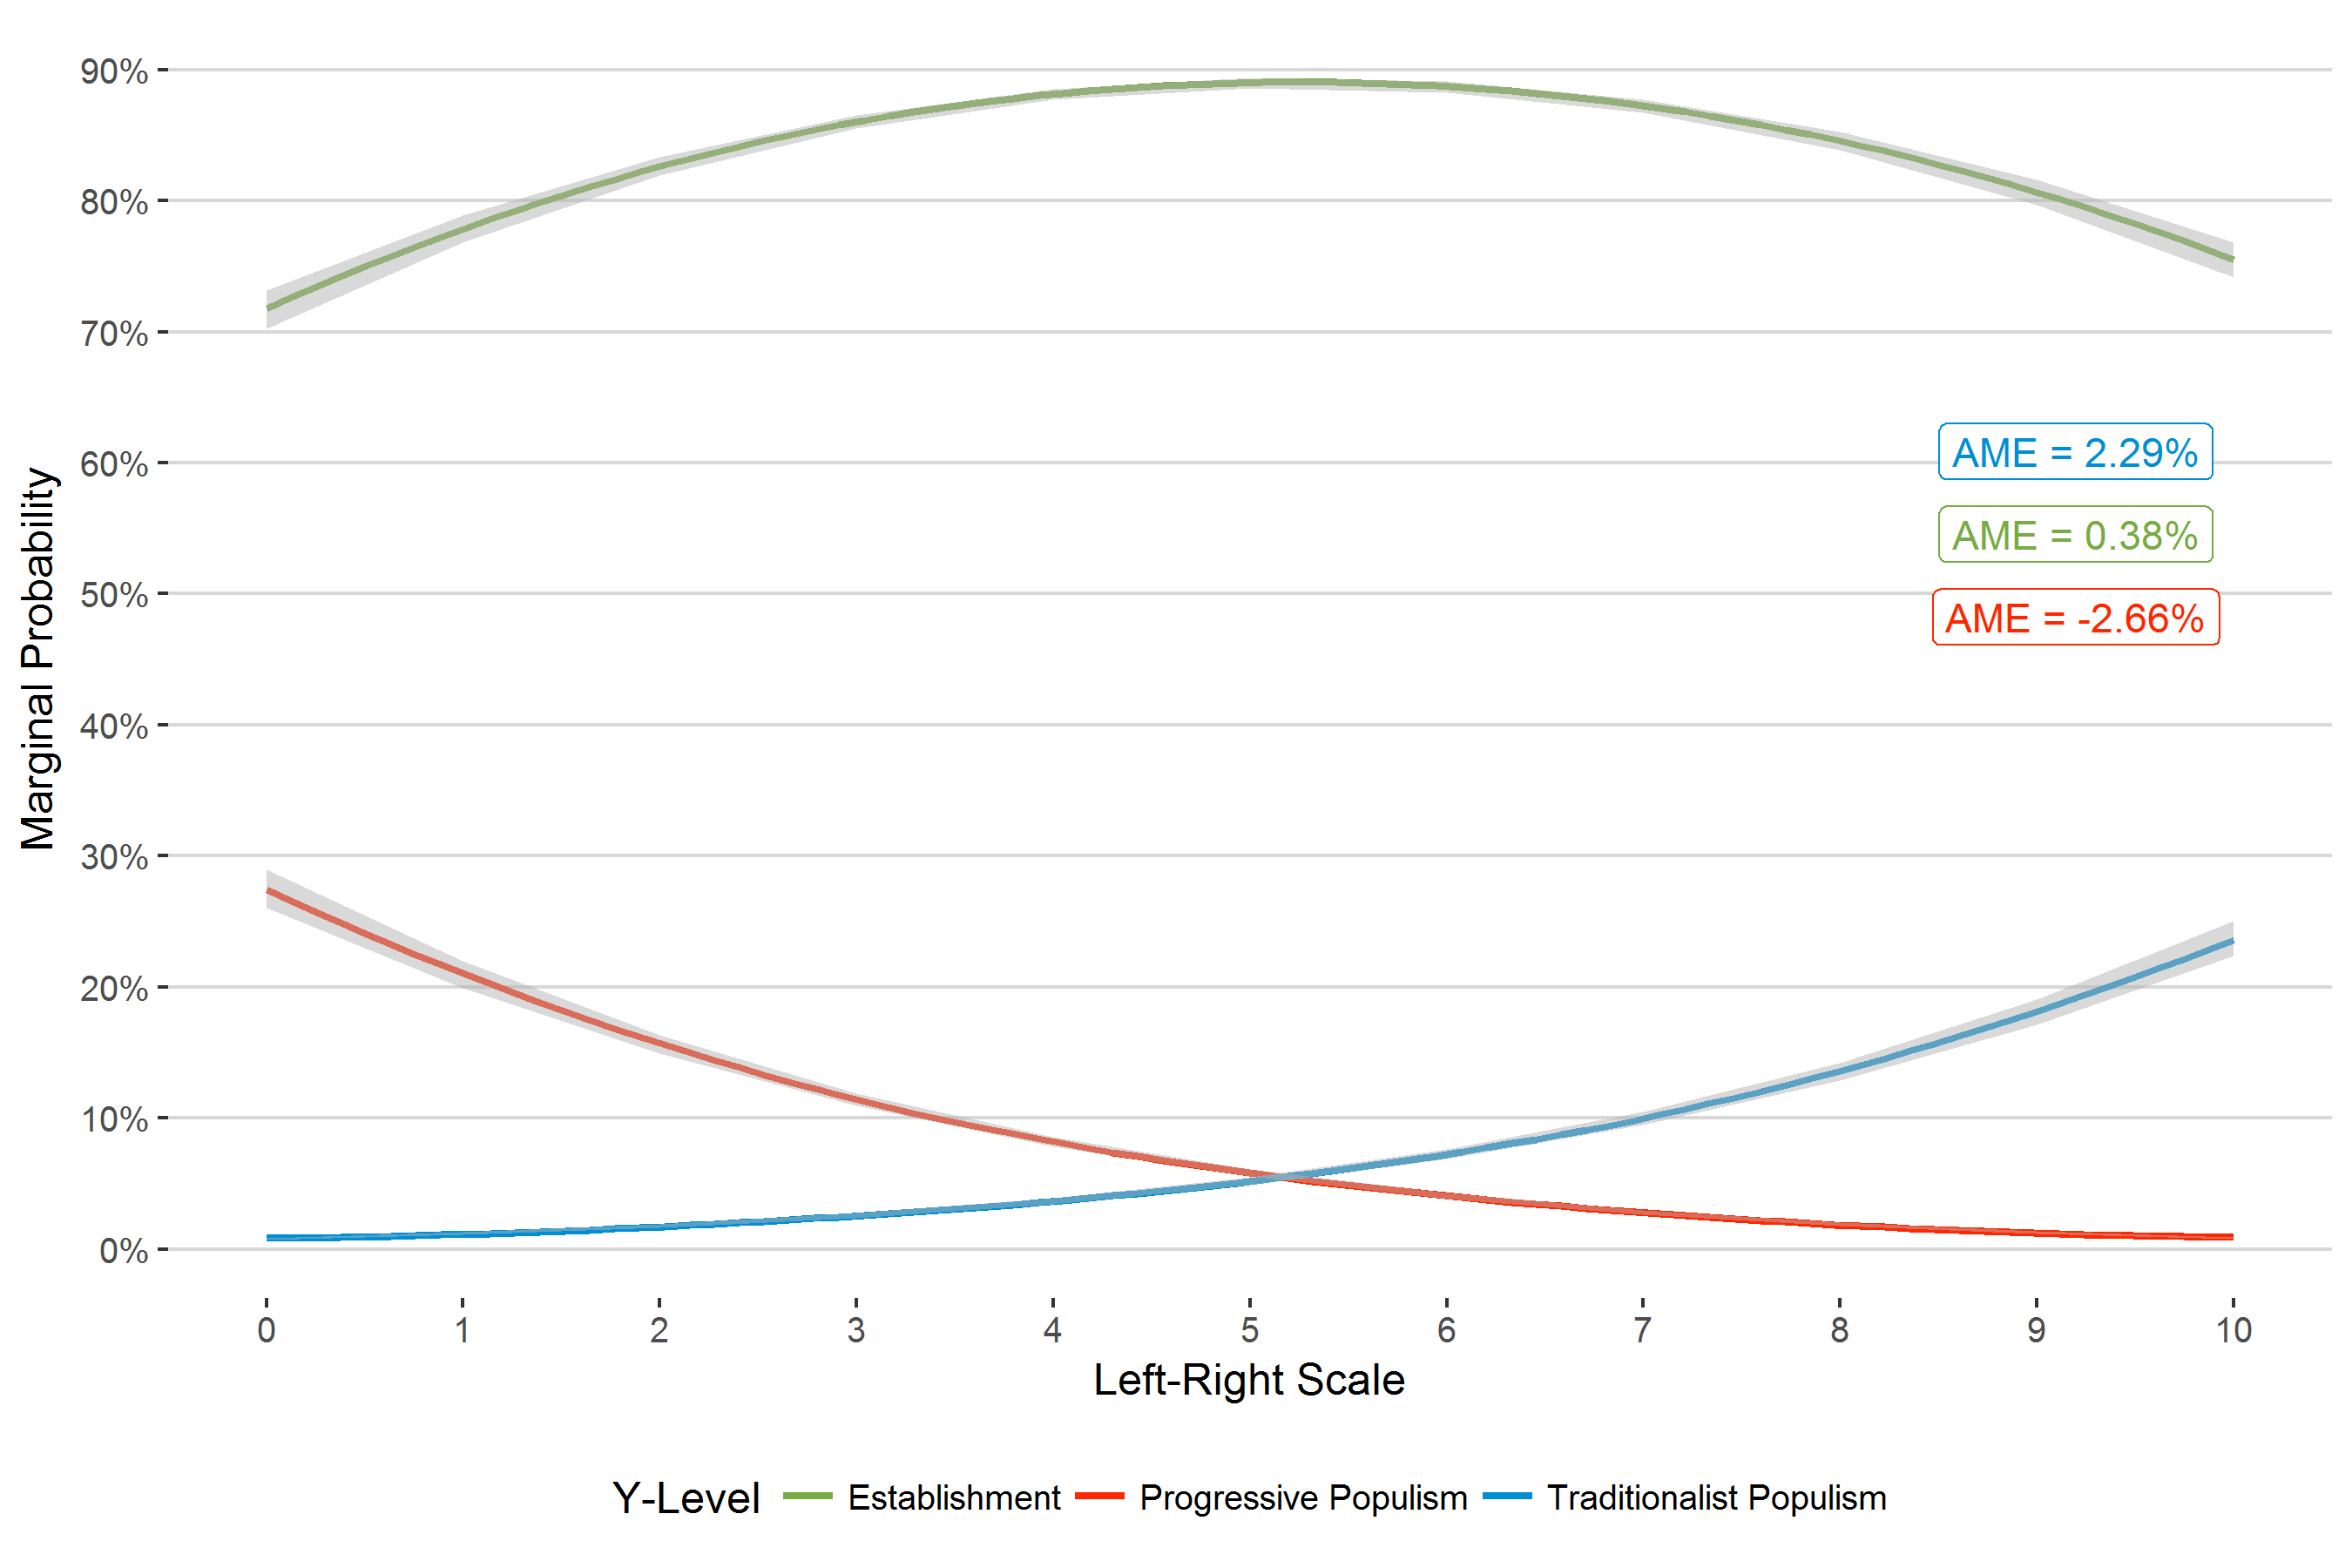
\includegraphics[width=\textwidth]{images/lrscale_probs.png}
	\flushright
	{\scriptsize Based on Model 4. Source: ESS Data Round 5 - 8; N = 68403. \par}
\end{figure}



% \setcounter{table}{1}
% \renewcommand{\thetable}{B\arabic{table}}
% \setcounter{figure}{1}
% \renewcommand{\thefigure}{B\arabic{figure}}


%---------------------------------------------------------------------------%
% Eigenständigkeiterklärung
%---------------------------------------------------------------------------%
\clearpage
\section*{Eigenständigkeitserklärung}
\vspace*{2cm}
\begin{center}
	\begin{minipage}[t]{0.8\textwidth}
		Hiermit versichern wir, dass wir die vorliegende Hausarbeit selbständig und nur mit den angegebenen Hilfsmitteln verfasst haben. Alle Passagen, die wir wörtlich als auch sinngemäß aus der Literatur oder aus anderen Quellen wie z. B. Internetseiten entnommen haben, sind deutlich als Zitat mit Angabe der Quelle kenntlich gemacht.
		
		\vspace*{60mm}
		Stuttgart, 20.03.2019
	\end{minipage}
\end{center}


\end{document}

